\documentclass[tikz,border=6pt]{standalone}
% Shared visual language for the original benchmark atlas.
\usepackage[T1]{fontenc}
\usepackage{lmodern}
\usepackage{amsmath,amssymb}
\usetikzlibrary{arrows.meta,calc,positioning,shapes.geometric,patterns,decorations.pathmorphing,backgrounds,fit}
\definecolor{ink}{HTML}{173948}
\definecolor{flow}{HTML}{167D9A}
\definecolor{control}{HTML}{A65217}
\definecolor{measure}{HTML}{70518A}
\definecolor{pale}{HTML}{EAF2F5}
\definecolor{muted}{HTML}{526571}
\definecolor{utility}{HTML}{2E8665}
\tikzset{
  every node/.style={font=\sffamily\small,text=ink},
  equipment/.style={draw=ink,line width=1pt,fill=pale,rounded corners=2pt},
  process/.style={draw=flow,line width=1.2pt,-{Latex[length=2.5mm]}},
  signal/.style={draw=control,line width=.8pt,dashed,-{Latex[length=2mm]}},
  util/.style={draw=utility,line width=1pt,-{Latex[length=2.2mm]}},
  dimension/.style={draw=muted,line width=.6pt,{Latex[length=1.7mm]}-{Latex[length=1.7mm]}},
  labelbox/.style={fill=white,inner sep=2pt,font=\sffamily\footnotesize,align=center},
  annotation/.style={font=\sffamily\footnotesize,text=muted,align=left},
  panel/.style={draw=ink!20,fill=ink!2,rounded corners=3pt,inner sep=6pt},
  instrument/.style={circle,draw=measure,fill=white,line width=.8pt,minimum size=8mm,inner sep=1pt,font=\sffamily\scriptsize,align=center},
  port/.style={circle,fill=flow,inner sep=1.6pt},
  box/.style={equipment,minimum width=3cm,minimum height=1cm,align=center},
}
\newcommand{\atlasheader}[3]{%
  \node[anchor=north west,font=\sffamily\bfseries\LARGE] at (0,0) {#1};%
  \node[anchor=north west,font=\sffamily\small,text=muted] at (0,-.75) {Paper section #2: \textit{#3}};%
  \draw[ink!25,line width=.7pt] (0,-1.25)--(26,-1.25);%
}
\newcommand{\atlasfooter}[1]{%
  \draw[ink!25,line width=.5pt] (0,-15.8)--(26,-15.8);%
  \node[anchor=north west,annotation,text width=25.8cm] at (0,-16) {#1\\Original explanatory drawing. Source: Kroll \& Schulte (2014), DOI: 10.1016/j.asoc.2014.08.034. Model variants are identified in the accompanying case sheet.};%
}

\begin{document}
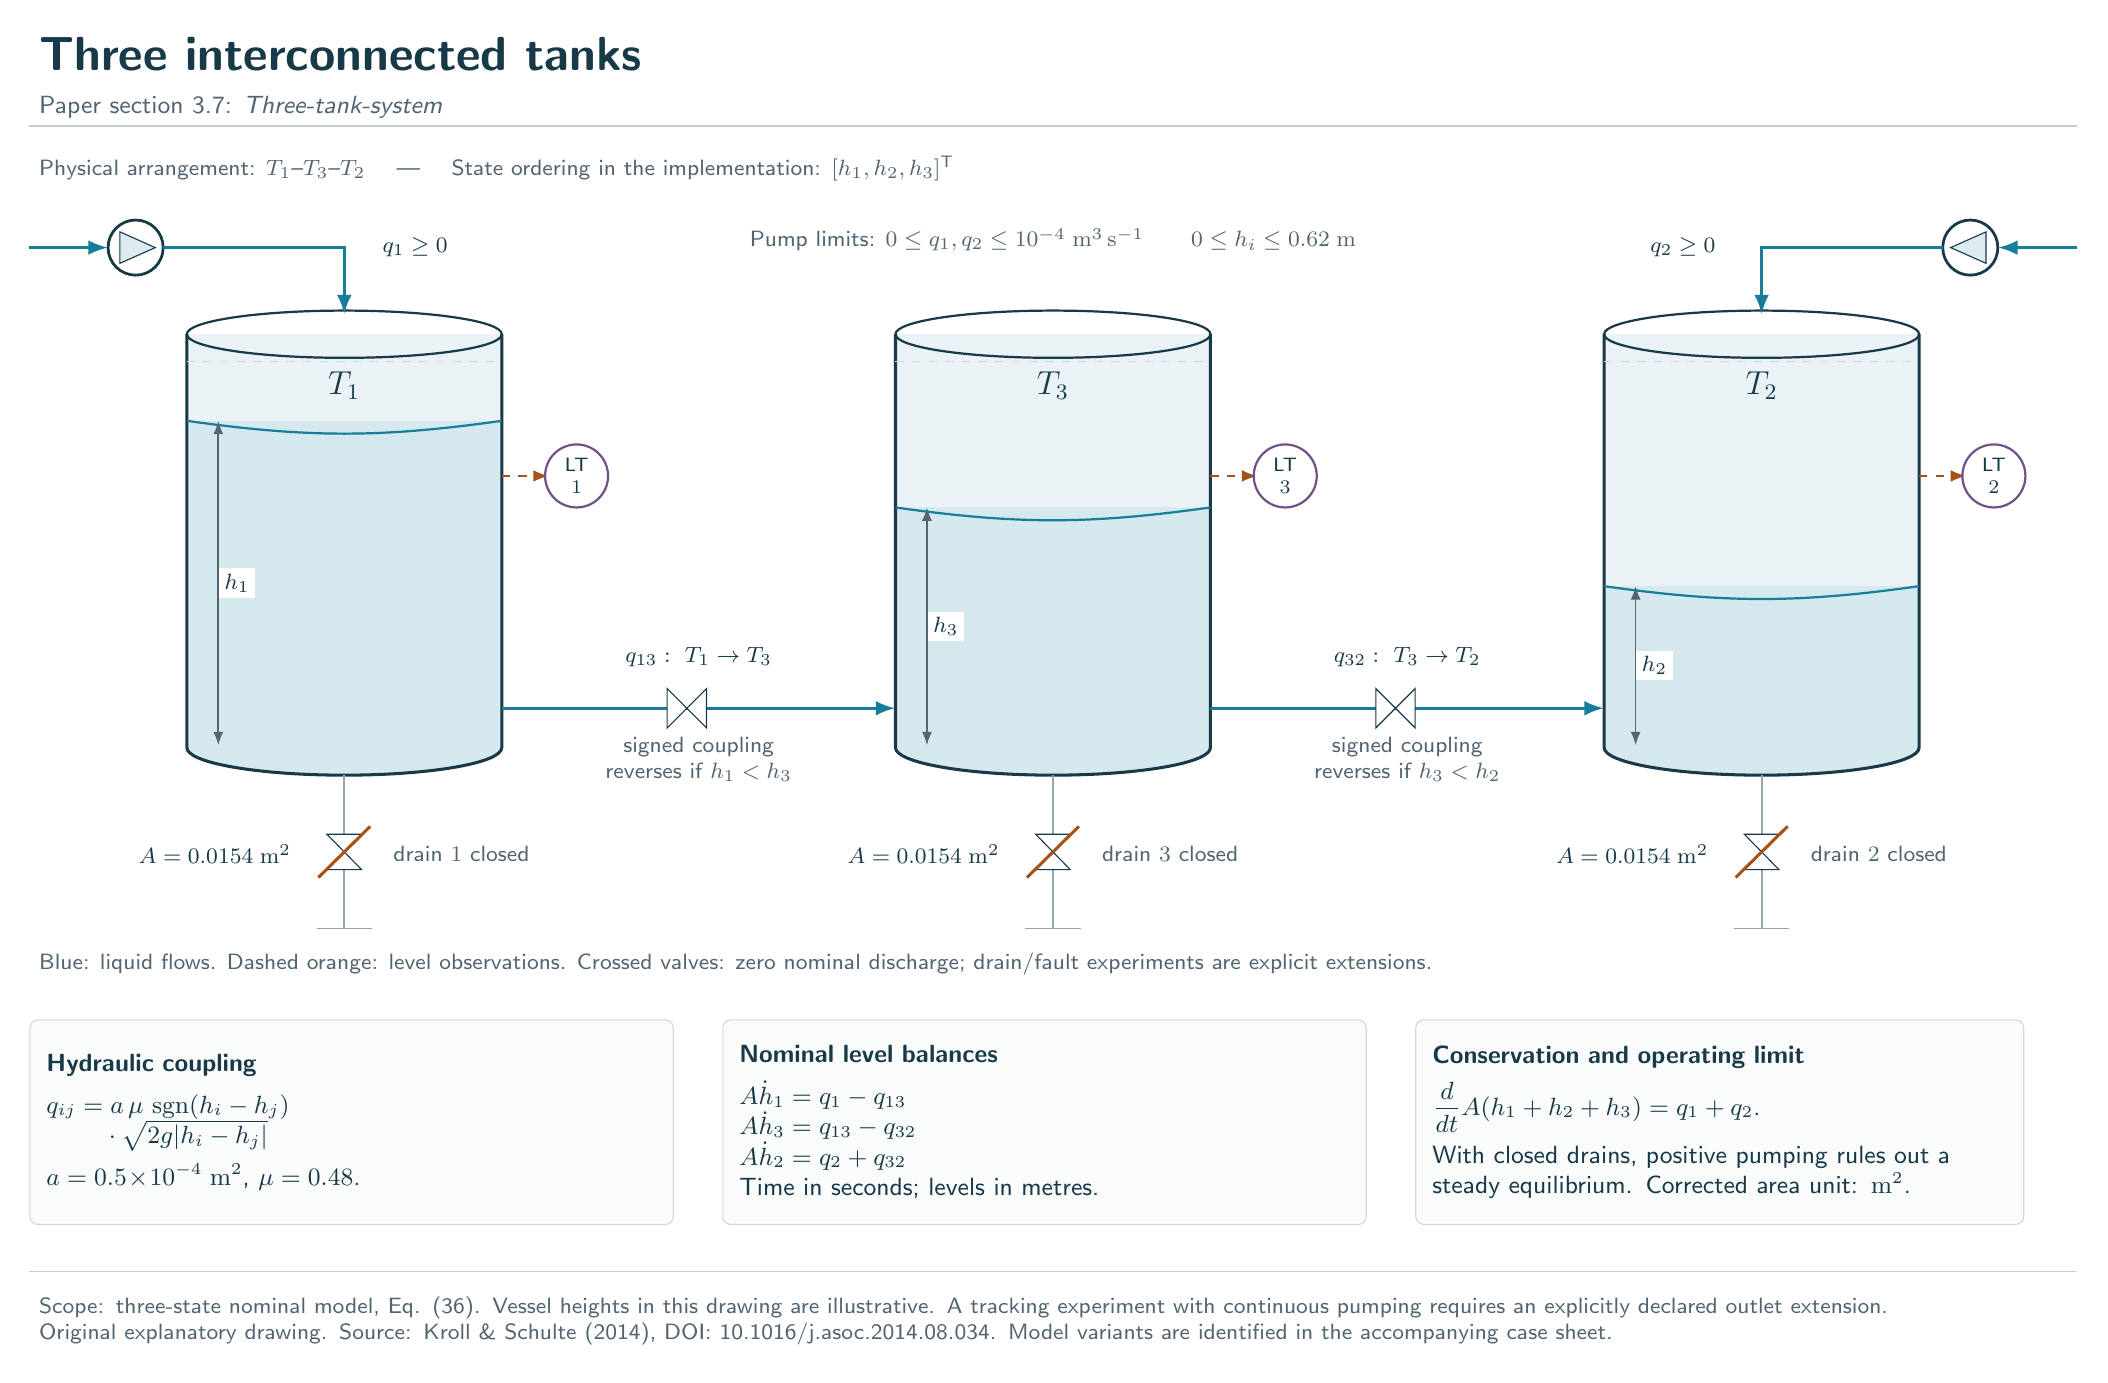
\begin{tikzpicture}[x=1cm,y=1cm]
\atlasheader{Three interconnected tanks}{3.7}{Three-tank-system}
\node[annotation,anchor=west] at (0,-1.8) {Physical arrangement: $T_1$--$T_3$--$T_2$ \quad | \quad State ordering in the implementation: $[h_1,h_2,h_3]^{\mathsf T}$};
% Free-surface vessels, with the intermediate tank physically in the middle.
\foreach \xl/\xr/\h/\name/\lev in {2/6/-5.0/1/1,11/15/-6.1/3/3,20/24/-7.1/2/2} {
  \path[fill=pale] (\xl,-3.9)--(\xl,-9.15) arc[start angle=180,end angle=360,x radius=2,y radius=.35] --(\xr,-3.9)--cycle;
  \path[fill=flow!18] (\xl,\h)--(\xl,-9.15) arc[start angle=180,end angle=360,x radius=2,y radius=.35] --(\xr,\h)--cycle;
  \draw[ink,line width=1.1pt] (\xl,-3.9)--(\xl,-9.15) arc[start angle=180,end angle=360,x radius=2,y radius=.35] --(\xr,-3.9);
  \draw[ink,line width=.8pt] ({(\xl+\xr)/2},-3.9) ellipse[x radius=2,y radius=.3];
  \draw[flow,line width=.8pt] (\xl,\h) to[out=-8,in=188] (\xr,\h);
  \draw[ink!20,dashed] (\xl,-4.25)--(\xr,-4.25);
  \node[font=\sffamily\bfseries\large] at ({(\xl+\xr)/2},-4.55) {$T_{\name}$};
  \draw[dimension] ({\xl+.4},-9.12)--node[labelbox,right] {$h_{\lev}$} ({\xl+.4},\h);
  \node[labelbox,anchor=east] at ({(\xl+\xr)/2-.6},-10.5) {$A=0.0154\;\mathrm{m^2}$};
}
% Two independent pumps feed the outer tanks.
\draw[process] (0,-2.8)--(1,-2.8);
\draw[equipment,fill=white] (1.35,-2.8) circle[radius=.35];
\draw[ink,fill=flow!15] (1.15,-3)--(1.6,-2.8)--(1.15,-2.6)--cycle;
\draw[process] (1.7,-2.8)--(4,-2.8)--(4,-3.65);
\node[labelbox] at (4.9,-2.8) {$q_1\geq0$};
\draw[process] (26,-2.8)--(25,-2.8);
\draw[equipment,fill=white] (24.65,-2.8) circle[radius=.35];
\draw[ink,fill=flow!15] (24.85,-3)--(24.4,-2.8)--(24.85,-2.6)--cycle;
\draw[process] (24.3,-2.8)--(22,-2.8)--(22,-3.65);
\node[labelbox] at (21,-2.8) {$q_2\geq0$};
\node[annotation] at (13,-2.7) {Pump limits: $0\leq q_1,q_2\leq10^{-4}\;\mathrm{m^3\,s^{-1}}$\quad\quad $0\leq h_i\leq0.62\;\mathrm m$};
% Bidirectional coupling: arrows define the positive sign, not a check valve.
\draw[process] (6,-8.65)--(11,-8.65);
\draw[ink,fill=white] (8.1,-8.4)--(8.6,-8.9)--(8.6,-8.4)--(8.1,-8.9)--cycle;
\node[labelbox] at (8.5,-8) {$q_{13}:\ T_1\rightarrow T_3$};
\node[annotation,align=center] at (8.5,-9.3) {signed coupling\\reverses if $h_1<h_3$};
\draw[process] (15,-8.65)--(20,-8.65);
\draw[ink,fill=white] (17.1,-8.4)--(17.6,-8.9)--(17.6,-8.4)--(17.1,-8.9)--cycle;
\node[labelbox] at (17.5,-8) {$q_{32}:\ T_3\rightarrow T_2$};
\node[annotation,align=center] at (17.5,-9.3) {signed coupling\\reverses if $h_3<h_2$};
% Level observations and calibrated vessel markings.
\foreach \xx/\id in {6/1,15/3,24/2} {
  \draw[signal] (\xx,-5.7)--({\xx+.6},-5.7);
  \node[instrument] at ({\xx+.95},-5.7) {LT\\$\id$};
}
% Closed drain branches are shown separately from the nominal flow network.
\foreach \xx/\id in {4/1,13/3,22/2} {
  \draw[ink!45,line width=.8pt] (\xx,-9.5)--(\xx,-11.45);
  \draw[ink,fill=white] ({\xx-.22},-10.25)--({\xx+.22},-10.7)--({\xx-.22},-10.7)--({\xx+.22},-10.25)--cycle;
  \draw[control,line width=1.1pt] ({\xx-.33},-10.8)--({\xx+.33},-10.15);
  \node[annotation,anchor=west] at ({\xx+.5},-10.5) {drain $\id$ closed};
  \draw[ink!45] ({\xx-.35},-11.45)--({\xx+.35},-11.45);
}
\node[annotation,anchor=west] at (0,-11.9) {Blue: liquid flows. Dashed orange: level observations. Crossed valves: zero nominal discharge; drain/fault experiments are explicit extensions.};
\node[panel,anchor=north west,text width=7.75cm,minimum height=2.6cm,align=left] at (0,-12.6) {\textbf{Hydraulic coupling}\\[4pt]
 $q_{ij}=a\,\mu\,\operatorname{sgn}(h_i-h_j)$\\$\hphantom{q_{ij}=}\cdot\sqrt{2g|h_i-h_j|}$\\[4pt]
 $a=0.5\!\times\!10^{-4}\;\mathrm{m^2}$, $\mu=0.48$.};
\node[panel,anchor=north west,text width=7.75cm,minimum height=2.6cm,align=left] at (8.8,-12.6) {\textbf{Nominal level balances}\\[4pt]
 $A\dot h_1=q_1-q_{13}$\\
 $A\dot h_3=q_{13}-q_{32}$\\
 $A\dot h_2=q_2+q_{32}$\\Time in seconds; levels in metres.};
\node[panel,anchor=north west,text width=7.3cm,minimum height=2.6cm,align=left] at (17.6,-12.6) {\textbf{Conservation and operating limit}\\[4pt]
 $\displaystyle\frac{d}{dt}A(h_1+h_2+h_3)=q_1+q_2$.\\[4pt]
 With closed drains, positive pumping rules out a steady equilibrium. Corrected area unit: $\mathrm{m^2}$.};
\atlasfooter{Scope: three-state nominal model, Eq. (36). Vessel heights in this drawing are illustrative. A tracking experiment with continuous pumping requires an explicitly declared outlet extension.}
\end{tikzpicture}
\end{document}
